\documentclass{acmsiggraph}                     % final
%\documentclass[annualconference]{acmsiggraph}  % final (annual conference)
%\documentclass[review]{acmsiggraph}            % review
%\documentclass[widereview]{acmsiggraph}        % wide-spaced review
%\documentclass[preprint]{acmsiggraph}          % preprint

%% Uncomment one of the five lines above depending on where your paper is
%% in the conference process. ``review'' and ``widereview'' are for review
%% submission, ``preprint'' is for pre-publication, and ``final'' is for
%% the version to be printed. The ``final'' variant will accept the 
%% ``annualconference'' parameter, which changes the height of the space
%% left clear for the ACM copyright information.

%% The 'helvet' and 'times' packages define the typefaces used for
%% serif and sans serif type in this document. Computer Modern Roman 
%% is used for mathematics typesetting. The scale factor is set to .92
%% to bring the sans-serif type in line with the serif type.

\usepackage[scaled=.92]{helvet}
\usepackage{times}
\usepackage{url}

%% The 'graphicx' package allows for the inclusion of EPS figures.

\usepackage{graphicx}

%% use this for zero \parindent and non-zero \parskip, intelligently.

\usepackage{parskip}

%% Optional: the 'caption' package provides a nicer-looking replacement
%% for the standard caption environment. With 'labelfont=bf,'textfont=it',
%% caption labels are bold and caption text is italic.

\usepackage[labelfont=bf,textfont=it]{caption}

%% If you are submitting a paper to the annual conference, please replace 
%% the value ``0'' below with the numeric value of your OnlineID. 
%% If you are not submitting this paper to the annual conference, 
%% you may safely leave it at ``0'' -- it will not be included in the output.

\onlineid{0}

%% Paper title.

\title{Page Curling in WebGL}

%% Author and Affiliation (single author).

%%\author{Roy G. Biv\thanks{e-mail: roy.g.biv@aol.com}\\Allied Widgets Research}

%% Author and Affiliation (multiple authors).

\author{Seth Samuel\thanks{e-mail: seth@visere.com}\\ Clibe}

%% Keywords that describe your work.

\keywords{webgl}

%%%%%% START OF THE PAPER %%%%%%

\begin{document}

\teaser{
  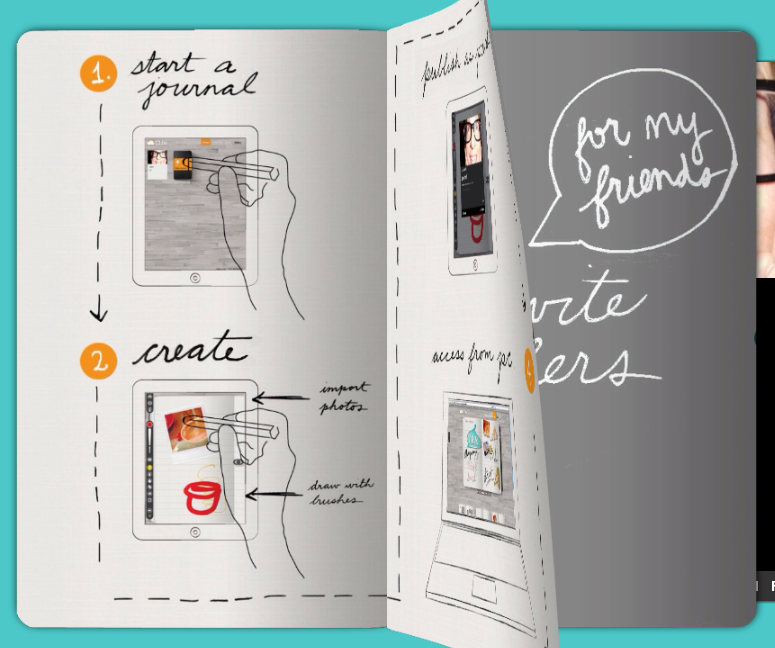
\includegraphics[width=1.5in]{pageturn.png}
  \caption{WebGL page turning in Chrome 18 for OS X.}
}

%% The ``\maketitle'' command must be the first command after the
%% ``\begin{document}'' command. It prepares and prints the title block.

\maketitle

%% Abstract section.

\begin{abstract}

\end{abstract}

%% ACM Computing Review (CR) categories. 
%% See <http://www.acm.org/class/1998/> for details.
%% The ``\CRcat'' command takes four arguments.

%\begin{CRcatlist}
%  \CRcat{K.6.1}{Management of Computing and Information Systems}%
%{Project and People Management}{Life Cycle};
%  \CRcat{K.7.m}{The Computing Profession}{Miscellaneous}{Ethics}
%\end{CRcatlist}

%% The ``\keywordlist'' command prints out the keywords.
%\keywordlist

\section{Introduction}

%% The ``\copyrightspace'' command must be the first command after the 
%% start of the first section of the body of your paper. It ensures the
%% copyright space is left at the bottom of the first column on the first
%% page of your paper.

 \copyrightspace

Our application implements the page turning algorithm specified by \cite{Lichan-Hong:2004fk} and implemented in OpenGL by \cite{Nuon:uq}.


\section{Implementation}
\subsection{Page Curling}
Page curling is a combination of a parameterized transformation approximating a cone  of varying width and position and a rotation about the y-axis.

The shape and position of the cone varies in three phases to simulate the severe curling that occurs at the start, more flat turning in the middle, and finally the wobble of settling onto the resting state. the attributes of the cone are calculated in Javascript then passed to WebGL shaders as uniforms.

The vertex shader calculates its projection onto the cone as a function of its two-dimensional position on the page's plane. 



\subsection{Two-Sided Textures}
A single mesh is used for each page, which has a different texture for each side. To determine the correct texture for a given fragment, a normal vector is passed for each vertex.

Singe each page is a parameterized plane, the vertex shader can calculate the position of vertices a small $\delta$ in either direction.

The normal vector is passed to the fragment shader, which determines if the normal is facing toward or away from the camera and picks the appropriate texture.
%\subsection{Queueing}
%Pages sit in a stack on either side of the active turning page, and are raised into the turning position as needed.


\section{Conclusion}

WebGL offers a powerful environment for 3D presentation on the web. While libraries such as three.js can offer significant advantages, implementation can still be challenging. 

\bibliographystyle{acmsiggraph}
\nocite{*}
\bibliography{template}
\end{document}
